% !TeX root = ../main.tex
% 原始章节：01-abstract.Rmd

\chapter{CPU芯片设计概述}\label{chap:01-overview}

\section{基本原理与结构简介}\label{sec:01-overview-001}

\subsection{经典计算机系统}\label{sec:01-overview-002}

现代计算机系统源自冯·诺依曼结构，并在应用需求的变化和工艺水平的提升下不断演变和发展。冯·诺依曼结构中的控制器和运算器逐渐整合为计算机系统中的中央处理器（CPU）部分，而输入、输出设备则通过北桥和南桥与中央处理器连接。随着技术的进步，中央处理器中的图形处理功能逐步分离出来，形成专用的图形处理器（GPU）。因此，现代计算机系统的硬件结构主要包括中央处理器、图形处理器、北桥和南桥等部分。

\textbf{中央处理器（Central Processing Unit, CPU）}是计算机的核心部件，主要包含控制器和运算器。随着计算机技术的发展，传统意义上的中央处理器在处理器芯片中表现为处理器核（Core），现代的处理器芯片上通常集成多个处理器核，以提高处理性能和效率。

\textbf{图形处理器（Graphics Processing Unit, GPU）}是一种专门用于2D和3D图形、视频处理、可视化计算和显示优化的处理器。作为人机交互的重要界面，GPU在计算机体系结构中的地位日益重要。除了图形处理外，GPU还被广泛用于科学计算和数据处理，加速复杂计算任务的执行。

\textbf{北桥（North Bridge）}是连接CPU和内存、显卡之间的重要桥梁，负责控制显卡和内存与CPU之间的数据交换。北桥位于CPU附近，直接与处理器相连，并通过总线与南桥连接。

\textbf{南桥（South Bridge）}负责管理计算机中带宽要求较低的外设，如硬盘、键盘和各种I/O接口。南桥通过北桥与CPU和内存进行数据交换，确保系统中各部分的协调工作。

现代计算机系统的一种早期架构是CPU-GPU-北桥-南桥结构。在这种架构中，计算机系统包含四个主要芯片，其中CPU（中央处理器）、北桥芯片和南桥芯片通常直接以芯片的形式安装或焊接在计算机主板上，而GPU（图形处理器）则以显卡的形式插入主板的扩展插槽中。

在CPU-GPU-北桥-南桥架构中，计算机的各个部件根据其速度和与处理器交换数据的频繁程度分别安排在北桥和南桥中。CPU通过处理器总线（也称系统总线）与北桥直接相连，北桥再通过南北桥总线与南桥相连，GPU一般通过显卡接口连接北桥。内存控制器集成在北桥芯片中，硬盘接口、USB接口、网络接口、音频接口以及鼠标、键盘等接口则放置在南桥芯片中。此外，北桥芯片还提供各种扩展接口用于连接其他功能卡。

采用该结构的计算机系统如图\ref{fig:structure-4part}所示。

\begin{figure}[htbp]
  \centering
  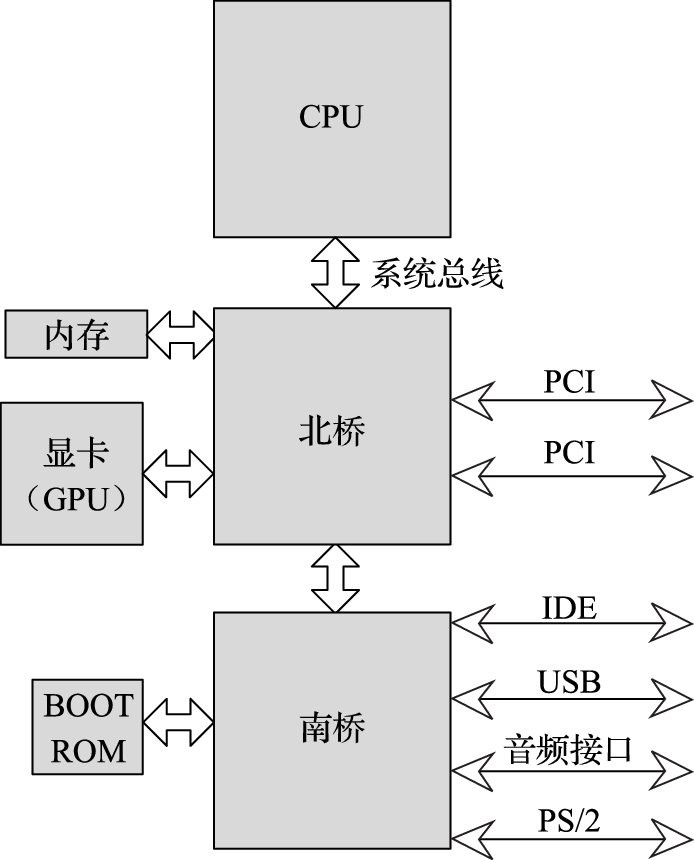
\includegraphics[width=0.5\linewidth]{assets/01/structure_4part.png}
  \caption{CPU-GPU-北桥-南桥结构}
  \label{fig:structure-4part}
\end{figure}

以英特尔奔腾处理器搭配的430HX芯片组为例，该芯片组采用了这种四片结构。其北桥芯片使用82439HX，南桥芯片采用82371SB，通过PCI总线扩展外接显卡，形成一个包括处理器在内的四片结构，构成计算机系统的核心部分。

\subsection{现代处理器 SoC 系统}\label{sec:01-overview-003}

片上系统（System on Chip，简称SoC）是一种单片计算机系统解决方案，它在单个芯片上集成了处理器、内存控制器、GPU以及硬盘、USB、网络等I/O接口，使得用户搭建计算机系统时只需使用单个主要芯片即可。SoC单片结构如图\ref{fig:soc}所示。

\begin{figure}[htbp]
  \centering
  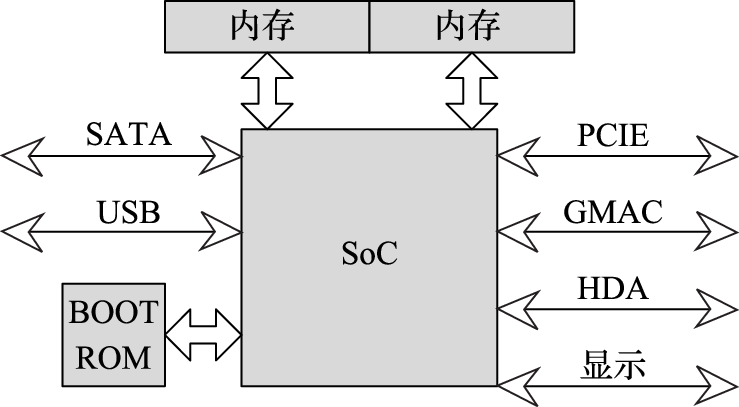
\includegraphics[width=0.5\linewidth]{assets/01/soc.png}
  \caption{SoC单片结构}
  \label{fig:soc}
\end{figure}

目前，SoC主要应用于移动处理器和工业控制领域。相比多片结构，单片SoC结构的集成度更高，功耗控制更加灵活，有利于系统的小型化和低功耗设计。然而，由于所有系统组件都集成在一个芯片上，SoC的系统扩展性较差，升级成本较高。随着技术的发展，封装基板上的互连技术不断进步，越来越多的处理器利用多片封装技术在单个芯片上集成多个硅片，以扩展芯片的计算能力或I/O能力。例如，AMD Ryzen系列处理器通过在封装上集成多个处理器硅片和I/O硅片，以提供针对不同应用领域的计算能力。龙芯3C5000L处理器则通过在封装上集成4个4核龙芯3A5000硅片，实现单片16核结构。

目前，主流商用处理器中，面向中高端领域的处理器普遍采用两片结构，而面向中低端及嵌入式领域的处理器则普遍采用单片结构。SoC单片结构最常见于手机等移动设备中。

\subsection{CPU芯片设计}\label{sec:01-overview-004}

在设计一款简单的现代系统级芯片（SoC）的过程中，一般需要达成以下核心目标：

\begin{enumerate}
\def\labelenumi{\arabic{enumi}.}
\tightlist
\item
  \textbf{处理器核心设计}
\end{enumerate}

\begin{itemize}
\tightlist
\item
  \textbf{架构选择}：一般选择一种简化的RISC（精简指令集计算）架构，如LoongArch精简指令集架构。该架构以其简单、高效和自主性著称，适合用于教育、研究和嵌入式系统。
\item
  \textbf{流水线技术}：采用流水线设计，以提高指令执行速度。流水线可以让处理器在一个周期内处理多条指令，提高吞吐量。
\item
  \textbf{缓存优化}：集成一级指令缓存（L1 I-cache）和数据缓存（L1 D-cache），以减少内存访问延迟，提高性能。
\item
  \textbf{虚拟地址翻译}：为支撑操作系统和应用程序的运行，设计虚拟地址翻译机制，支持虚拟内存管理。
\end{itemize}

\begin{enumerate}
\def\labelenumi{\arabic{enumi}.}
\setcounter{enumi}{1}
\tightlist
\item
  \textbf{外设设计}
\end{enumerate}

\begin{itemize}
\tightlist
\item
  \textbf{输入输出接口}：需要支持包括多种常见的I/O接口，如UART、SPI、I2C、GPIO等，确保与外部设备的兼容性和互操作性。
\item
  \textbf{内存控制器}：集成内存控制器，选择性支持SDRAM、DDR等类型内存，确保高效的数据存取。
\item
  \textbf{图形处理器}：集成简单的图形处理器，支持基本的图形处理需求，以提高用户体验。
\end{itemize}

\begin{enumerate}
\def\labelenumi{\arabic{enumi}.}
\setcounter{enumi}{2}
\tightlist
\item
  \textbf{系统互连}
\end{enumerate}

\begin{itemize}
\tightlist
\item
  \textbf{总线架构}：采用AMBA（Advanced Microcontroller Bus Architecture）等高效的总线架构，确保处理器核心和外设之间的高效数据传输。
\item
  \textbf{DMA控制器}：集成DMA控制器，支持大块数据的高速传输，减轻处理器核心的负担，提高系统整体效率。
\end{itemize}

\section{芯片实现流程简介}\label{sec:01-overview-005}

芯片实现流程是一系列复杂步骤的集合，包括从定义到设计再到物理实现、流片、封装、系统搭建等，涵盖了从概念到最终产品的转变。本节主要从流程的角度去概要性的描述如何实现CPU从概念提出到具体应用落地，整体流程示意如图\ref{fig:chip-flow1}所示，可分为前端设计与综合实现、后端物理实现与验证、流片制造与测试三个部分。需要注意的是如果在某个验证环节（比如功能仿真）没有通过，则需要回到前面设计（HDL设计或后端布局布线设计等）的某一步重新执行。下面针对这三个部分展开介绍。

\begin{figure}[htbp]
  \centering
  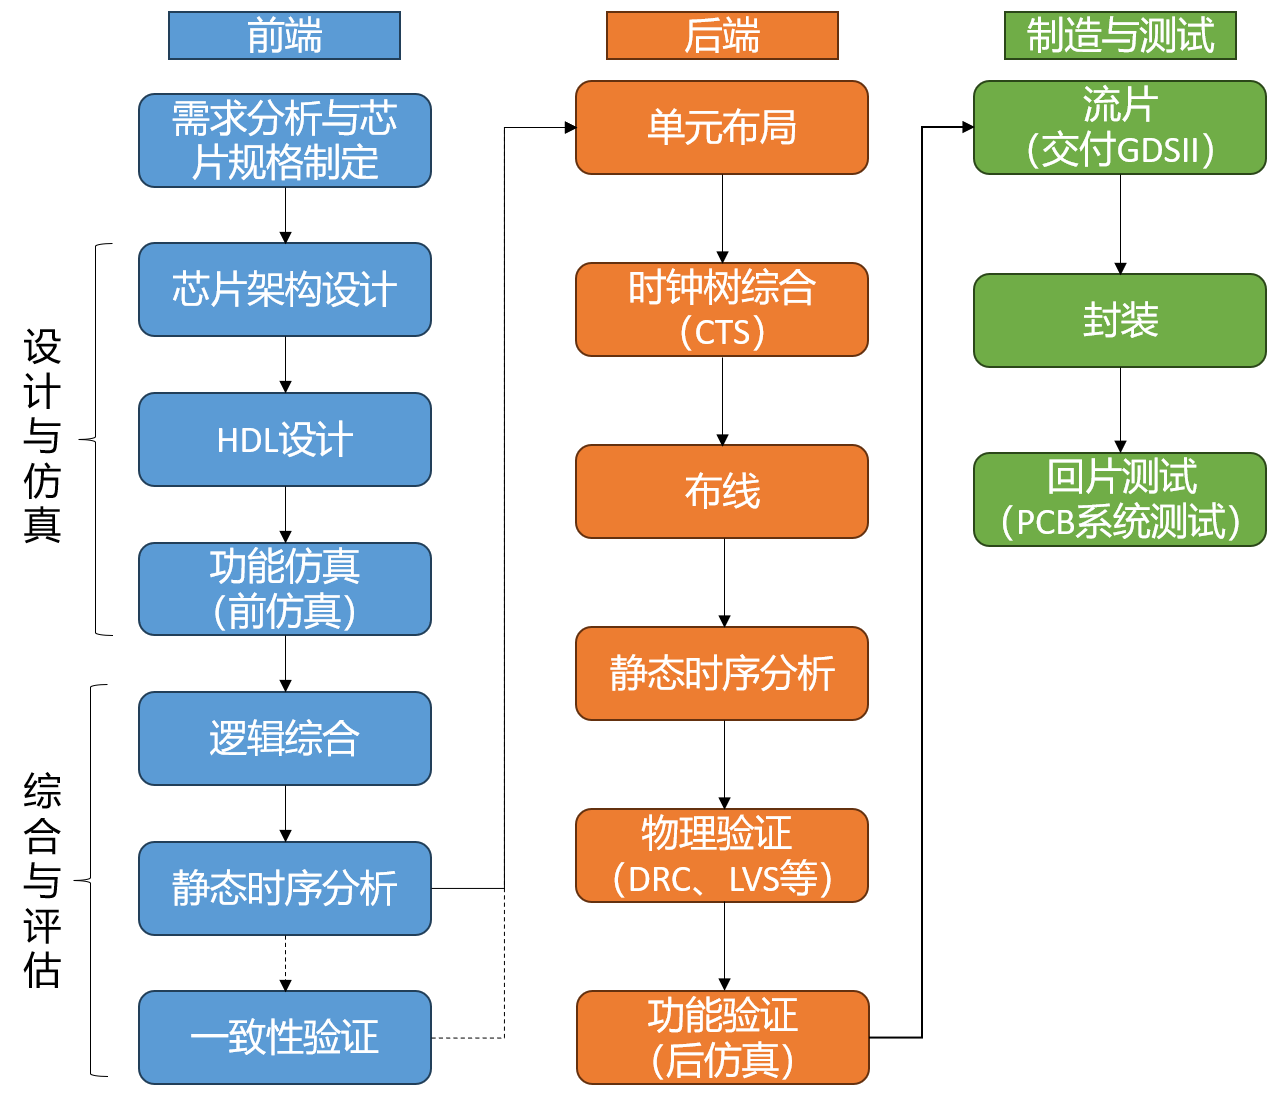
\includegraphics[width=0.5\linewidth]{assets/01/芯片实现流程.png}
  \caption{芯片实现流程示意图}
  \label{fig:chip-flow1}
\end{figure}

\subsection{芯片规格定义与设计仿真实现}\label{sec:01-overview-006}

首先芯片实现需要完成设计部分：

\begin{itemize}
\tightlist
\item
  \textbf{需求分析与规格制定}：首先一款处理器芯片，需要明确其应用场景，根据场景来确定需求，完成整体设计规格书（SPEC）。比如应用在嵌入式的处理器与应用在服务器的处理器二者对于性能、功能场景的需求差异就比较大。因此需要进行需求分析与规格制定。
\item
  \textbf{芯片架构设计}：一般对于大型负责芯片项目设计（比如现代CPU），都会在详细设计前进行系统架构设计。通过System C、Matlab等工具完成对架构的分析与验证，以确保在系统架构上不出现问题。
\item
  \textbf{HDL设计}：即通过硬件描述语言将所设计的架构进行实现。这一步一般通过VerilogHDL或VHDL来进行编写。需要注意的是此时编写的代码必须是可综合的RTL代码。目前也有一些其他更高级、敏捷的硬件描述语言在推广中，如chisel、SpinlHDL等，这些语言抽象层级更高，实现起来更加便捷。本教材中的部分CPU设计内容就是通过chisel来实现的。
\item
  \textbf{功能仿真}：此时也叫前仿真。即在HDL编写完成后需要进行仿真验证。这一步一般通过编写testbench，使用EDA仿真工具完成。当然在模块化设计的过程中，一般会每实现一个模块就要进行一次仿真，并根据仿真发现的问题进行修改设计中的错误。因此HDL设计与功能仿真这两步一般也可以放在一些来统称为HDL实现。在一些大型芯片项目中，仿真验证工作是占用时间最长的一部分。
\end{itemize}

在功能仿真完全正确之后，可以进行下一步，逻辑综合。

\subsection{芯片设计逻辑综合与评估验证}\label{sec:01-overview-007}

前面几步都属于设计的部分，本教材也着重讲述CPU设计部分的内容。在设计完成后，并不意味着能够将硬件代码完全冻结（即不再对HDL代码进行更改），因为时序等还没有进行收敛测试。下面进行几步来完成此事：

\begin{itemize}
\tightlist
\item
  \textbf{逻辑综合}：这一步主要是将HDL编写的RTL代码映射为可用于后端过程的门级网表。这一过程旨在决定电路的门级结构，寻求时序与面积以及功耗的平衡，同时增强电路的测试性。从这一步开始到后面的内容都将有具体工艺的参与。
\item
  \textbf{静态时序分析}：这一步主要用于分析电路时序是否满足要求，是用于时序signoff的关键步骤。一般EDA在进行逻辑综合时，也会进行一些静态时序分析（STA），但其准确性一般不如专门做STA的工具Synopsys PrimeTime工具。通过静态时序分析来分析电路的关键路径，分析硬件设计是否满足时序要求。若不满足则需要返回到HDL设计，通过针对关键路径优化等策略使时序收敛。
\item
  \textbf{一致性验证}：该步骤主要用于验证综合后的网表文件与综合前的HDL设计文件的功能一致性，以保证逻辑综合过程没有改变HDL所描述的电路功能。
\end{itemize}

在通过静态时序分析以及通过其他约束条件下收敛之后，网表文件就可以传递到下一步进行后端操作。

\subsection{芯片后端物理实现与验证}\label{sec:01-overview-008}

芯片后端物理实现主要包括布局规划、电源规划、时钟树综合、布线等步骤。验证包括芯片静态时序分析、功耗验证、物理验证等过程。

\begin{itemize}
\tightlist
\item
  \textbf{单元布局}：主要作用是将设计好的网表文件进行单元器件的摆放，一般布局包括布局规划、电源规划以及自动布局等步骤。布局规划即芯片尺寸规划、IO规划、macro摆放、物理单元插入等步骤。电源规划即将电源模块进行位置规划。自动布局即在完成规划的基础上，由EDA工具自动进行布局操作，以满足设定的时序、功耗、面积等条件或进行相应的优化。
\item
  \textbf{时钟树综合}：时钟树综合（CTS）是在物理设计中为芯片中的时钟信号构建一棵优化的树状结构，确保时钟信号能够同时到达所有时序单元，最小化时钟偏移和抖动，优化时序和功耗，从而确保芯片的时序收敛性和整体性能。
\item
  \textbf{布线}：一般分为全局布线与详细布线、布线优化等步骤。全局布线是指在芯片的全局范围内确定信号的布线路径和大致走线方向；详细布线是在全局布线的基础上，为每一根信号线分配具体的布线层、布线路径和布线宽度；在完成初步的详细布线后，进行布线优化以改善时序、降低功耗、减少信号干扰和提高芯片的制造良率。布线过程一般是EDA自动完成的，但有些情况可能需要手动布线。
\item
  \textbf{静态时序分析}：此时的时序分析有了更准确的单元延迟结果，此时的分析结果是更加精准的。这一步也用于芯片的时序signoff。
\item
  \textbf{物理验证}：主要验证设计规则检查（DRC）、电气规则检查（ERC）、布局与布线等效性验证（LVS）、信号完整性检查（SI）、功耗分析（Power Analysis）等。这些验证内容涵盖了从物理布局到电气性能的各个方面，确保芯片在功能、性能、制造和可靠性上都能达到预期要求。通过全面的物理验证，可以大大降低芯片流片失败的风险，确保芯片能够顺利进入量产阶段。
\item
  \textbf{功能验证}：这一步主要用于在版图实现后对电路功能的测试，这一步的测试条件就变得更加苛刻。再完成上述所有内容之后，后端就产出了GDSII文件用于发送给晶圆厂用于制造。
\end{itemize}

\subsection{芯片流片、封装与回片测试}\label{sec:01-overview-009}

一般芯片在回片前就需要完成对PCB测试系统的搭建。

\begin{itemize}
\tightlist
\item
  \textbf{流片制造}：在正式流片前，设计团队和客户要对设计进行最终签核（Sign-off），确保所有的设计规则、时序、信号完整性等问题都已经解决；制造厂根据设计文件制作光罩（mask），使用光罩在晶圆上进行光刻、刻蚀、掺杂、金属化等步骤，逐步将设计实现为物理晶体管、互连和其他器件。最终完成一款裸片（Die）的制造。
\item
  \textbf{芯片封装}：封装是指将制造完成的裸片（Die）进行物理保护并提供电气连接的过程。封装后的芯片可以安装到电路板上并与外部环境进行交互。一般封装会经过晶圆切割、晶圆测试、贴片封装、引线键合、倒装芯片（可选）、封装密封、测试、打标检查等步骤，最终出货给客户。
\item
  \textbf{测试系统搭建}：一般芯片完成封装后需要搭建测试系统来完成最终的功能、性能测试。包括外围电路设计、外设搭建、PCB绘制等。有时也会在回片前使用一个FPGA来模拟芯片功能进行系统的测试。
\item
  \textbf{芯片系统测试}：通过将芯片安装在测试电路板上，实现板上测试，最终验证芯片的功能、性能等特征。
\end{itemize}

通过以上介绍，完成了对一般数字芯片从设计到后端实现再到制造、回片测试各个环节的介绍。本教材将带领读者学习CPU芯片从架构设计到验证再到实现的各个细节，以真正让读者全面了解与掌握整个CPU芯片实现从理论到实践的核心知识。无论是初学者还是具有一定经验的工程师，本书都将提供系统的指导和实用的技巧，助力在CPU芯片设计过程中实现创新与突破。
